\chapter{Implementation}
\label{ch:Implementation}
This chapter describes the details of the implementation of the prototype and the analysis of the data collected during the studies.
To implement the prototype, Arduino software was developed to measure temperature sensor values and IMU data and store them on a microSD card with a timestamp.
Implementation details for evaluating and analyzing the collected data are described afterwards.

\section{Prototype}
The prototype is controlled by OpenEarable, which was programmed to be controlled via Arduino code. 
An Arduino Nano33 BLE is built into the OpenEarable, which facilitates customization. 
The main task of the prototype is to collect data from the temperature sensors and an IMU, and store it in a CSV file on the SD card, which has its own slot in the OpenEarable. 
Similar to traditional Arduino code, the prototype code consists of a \texttt{setup()} and a \texttt{loop()} method.
A general overview of the code can be visually seen in Figure \ref{fig:ch:Implementation:ArduinoCodeProcedure}.

\begin{figure}[!t]
    \centering
    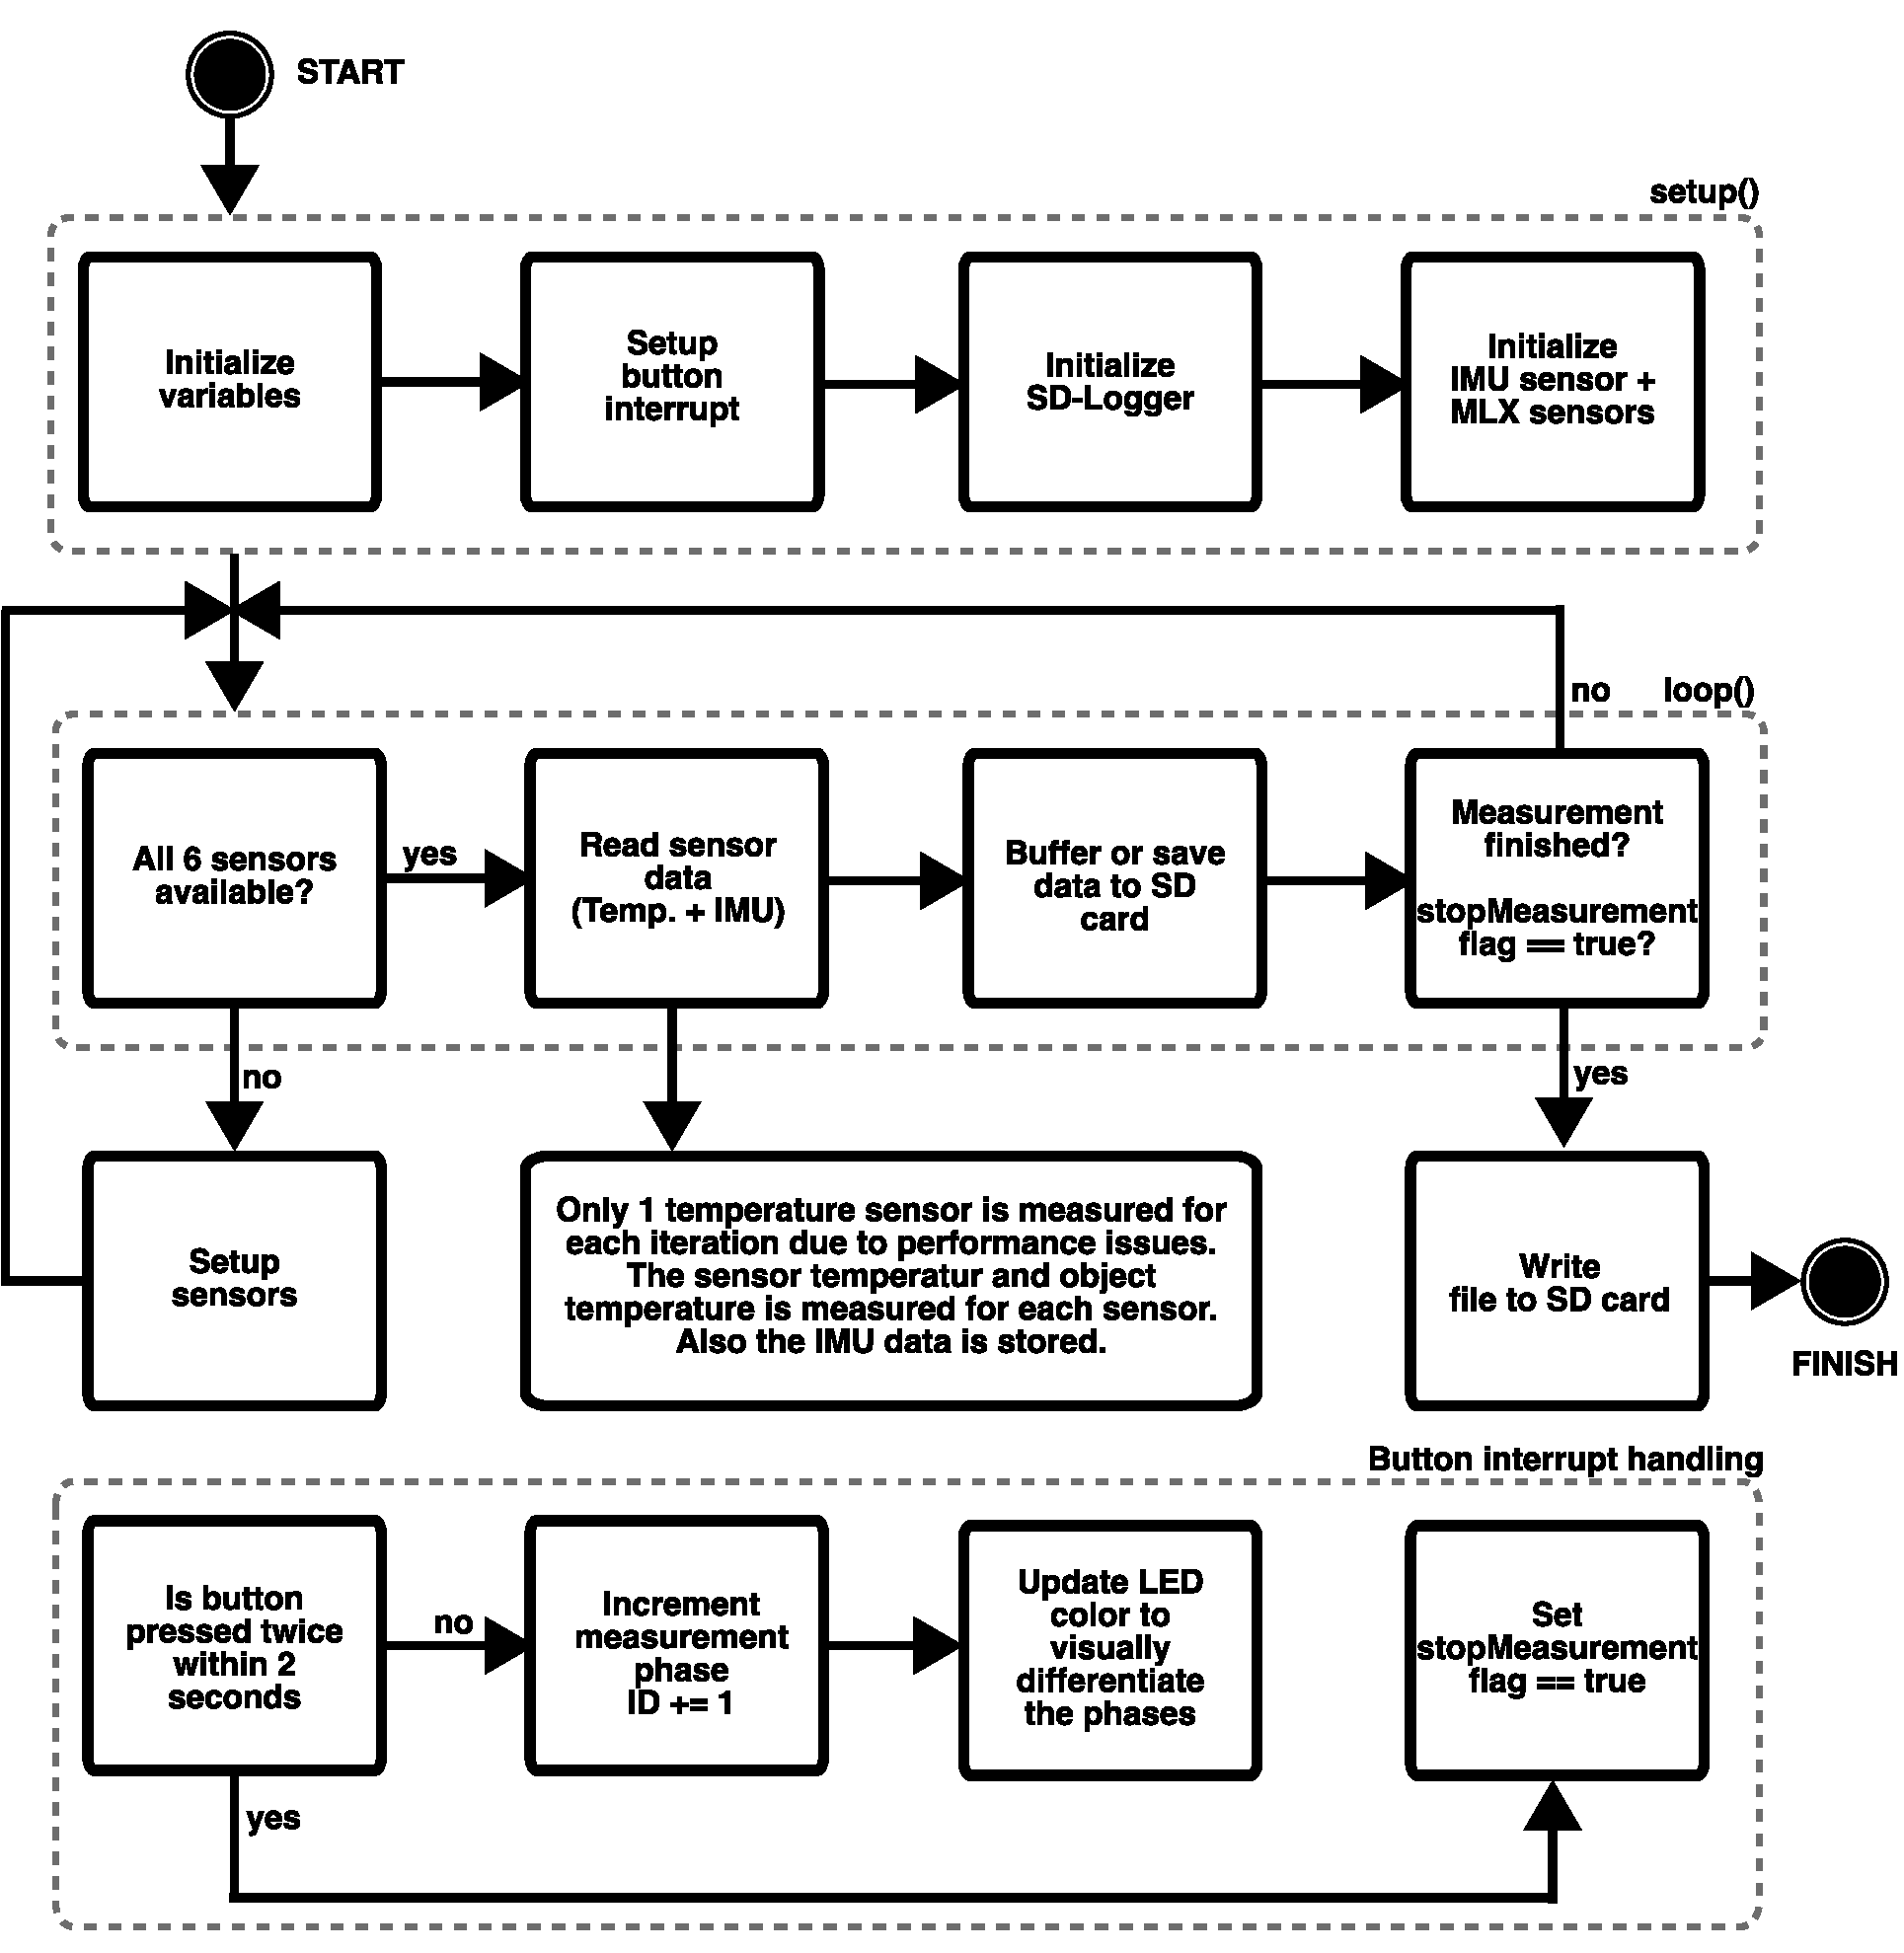
\includegraphics[width=\textwidth]{thesis-doc/images/ArduinoCodeProcedure2.pdf}
    \caption{Sequence of the behavior of the prototype. Using the ArduinoIDE, the code is written in $c++$ and flashed to the OpenEarable. The code includes the usual "setup()" and "loop()" functions and their behavior to create the dataset for the two studies.
This results in a csv file that contains all the information.}
    \label{fig:ch:Implementation:ArduinoCodeProcedure}
\end{figure}

In the \texttt{setup()} method, all the required components are initialized. These include the sensors, the IMU, the SD card logger and the key interrupt. The latter is used to ensure that a measurement is terminated, if the key is pressed twice within two seconds. 
If the key is pressed once, the phase is changed. 
When the sensors are initialized, a \texttt{Wire} connection is made and the multiplexer is triggered.
The multiplexer is crucial when reading out the sensors, because each sensor is addressed with the same address.
All temperature sensors are connected to the multiplexer and are addressed one after the other to read out the temperature value.
This is possible because the multiplexer always switches through one output and thus all sensors can have the same address.

In addition to the regular operations in the \texttt{loop()} method, the code contains functions for handling keystrokes. A key press is detected using an interrupt. As soon as the key is pressed, a function is started that checks whether the key has already been pressed within the last two seconds. If this is the case, the data acquisition of sensor data and IMU data is stopped and the SD card with the collected data is written.

One of the main tasks is to read data from the MLX90632 sensors and the IMU sensor. 
For this, the multiplexer is always switched to the respective sensor and the value is read and persisted via the modified library "Protocentral\_MLX90632".
The library was strongly modified to enable a faster measurement. 
This is necessary because additional motion data should be recorded.
The IMU sensor, built directly into the OpenEarable, provides accelerometer, gyroscope and magnetometer data.

The collected data from one iteration of the \texttt{loop()} function is then written to the SD card. Each line represents one pass of the \texttt{loop()} function and contains one of the 6 temperature sensor values and the 9 IMU data as well as a time value and an ID.
Thus the 6 temperature sensor values are distributed in 6 lines. 

Furthermore the library "Protocentral\_MLX90632" was adapted. In the original library, the \texttt{getObjectTemp()} function waits for the temperature value to become available by waiting in a \texttt{while} loop for a register value to be set indicating newly available data. This resulted in an unacceptably long waiting time because the update rate per sensor is 2 Hz. 
During this time, no IMU data signal can be read due to the \texttt{while} loop present in the library, as the Arduino Nano33 BLE does not allow parallelism. 
To fix this problem, the check to see if new data is available is ignored. 
Instead, the temperature value is read in each loop iteration. 
As a result, the temperature value may not have updated yet. 
However, the sampling rate is so high that this does not affect the final result.
The IMU data needs a sampling rate of at least 50Hz to make significant statements about the motion. 
To achieve this, only one sensor value per iteration was read out to achieve the performance. 
Additionally, the code had to be optimized several times for performance reasons, ranging from removing \texttt{for} loops to storing data in strings, instead of arrays. 
Finally, a sampling rate of $50Hz$ of IMU data and a sampling rate of $8.3Hz$ of sensor values has been achieved.
Since the temperature sensors have an update rate of $2Hz$, some consecutive sensor values are the same, but no measured sensor value is lost.
A snippet of the final result of the csv file can be taken from Figure \ref{fig:implementation:raw_csv_content_snippet}. Please note that the temperature of the sensor itself is also stored, but is not shown here due to space limitations.

\begin{figure}[!t]
    \centering
    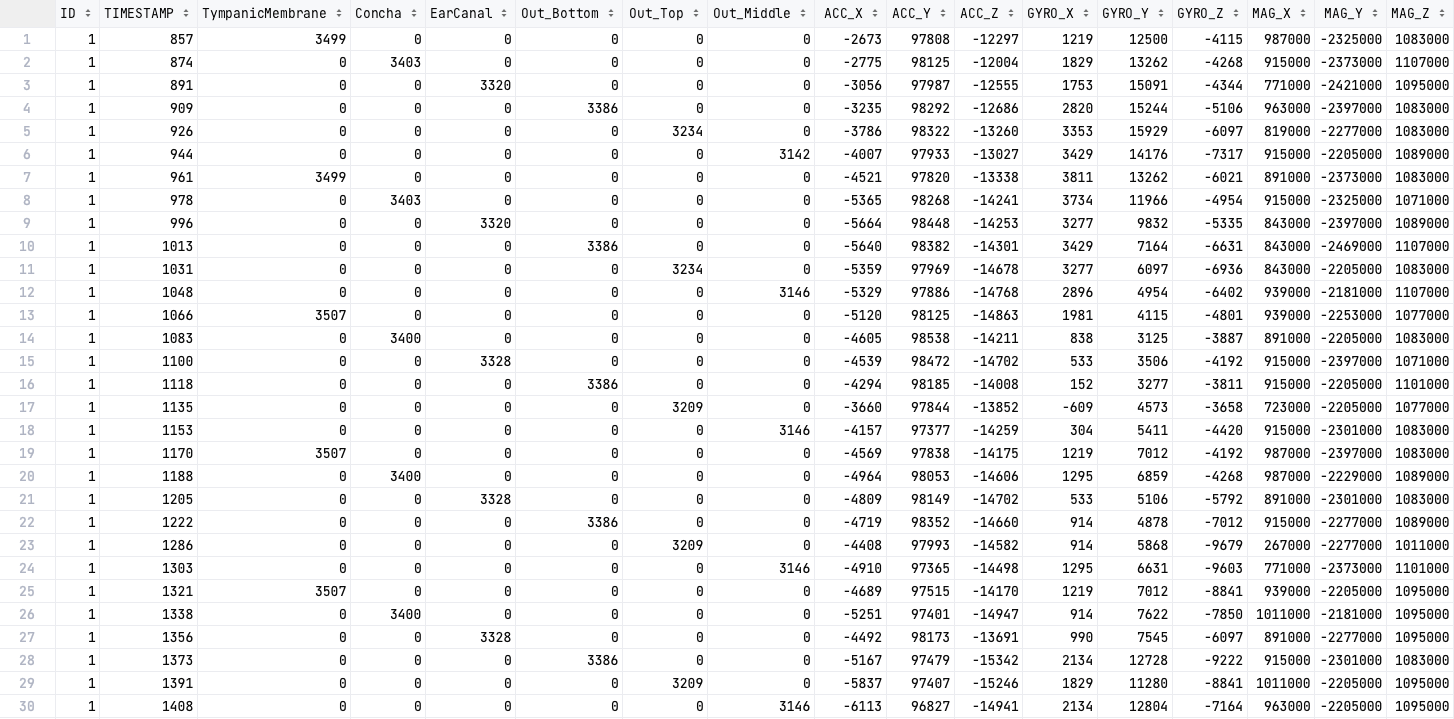
\includegraphics[width=\textwidth]{thesis-doc/images/prototype/MeasurementRawDataSnippet.png}
    \caption{Snippet of the resulting csv-file from study 1 of subject 10. The temperature values were multiplied by 100 to store the values as integer and to have two decimal places. The IMU data were each multiplied by 10000 to retain the information over three decimal places. The timestamp is given in milliseconds, the "ID" defines the current phase the measurement is into.}    
    \label{fig:implementation:raw_csv_content_snippet}
\end{figure} 

\section{Sensor Calibration Implementation in Arduino}
The calibration was implemented using the Arduino platform, modifying the library for the MLX90632 sensors to introduce an emission factor of $0.98$ according to the sensor datasheet. 
This value is optimized to measure the temperature of the human body and was also used for the metal plate during calibration. 
This emission factor allows the system to account for the natural variability of thermal radiation between different materials and provide a standardized reading that is consistent across environments.

\section{Study Analysis}
A pipeline was created for each of the analyses of Study 1 and Study 2. 
The code of the two studies is located in the Git directory in the folder "codingStuff/studyAnalysis", respectively in the folders "study1" and "study2".
The pipeline first reads all the recorded data into a Pandas data frame and generates the results for the different hypotheses.
For each hypothesis, a file: "hypothesisX.py" exists, where the "X" stands for the number of the hypothesis. 
This is called in the pipeline and all results, either output or plots, are saved in the "target" folder or printed to the console.

\subsection{Analysis of Study 1}
The analysis of the first study is stored in the file "study1\_pipeline.py". 
Running this file starts a pipeline to evaluate all hypotheses.
At the beginning of the pipeline is the \texttt{AnalysisPipeline} class, which specifies the data folders and destination folders as class attributes. 
This serves as a representation of the pipeline and manages the complete pipeline.
In addition, the class holds the ground truth temperature measured by all subjects in the class attribute \texttt{ground\_truth\_temps}.
Then, the function \texttt{process\_directory} is called, which stores all the records of each subject's study in the class attribute \texttt{all\_temp\_data}.
For this purpose, an object of class \texttt{TemperatureData} is created for each individual record.
This file is stored in the "src" folder, as are all other files.
Among other things, this object stores the raw data of the sensor values, as well as the ground truth value, which was previously stored in \texttt{ground\_truth\_temps} of all subjects.
Since the temperature values were stored as \texttt{Integer} and multiplied by 100 in the csv file, the temperature values were also divided by 100 when persisted.
Since only one temperature sensor value is stored per measurement and the other 5 sensor values are set to 0, they are also set to "NaN", which greatly simplifies the subsequent recording of the data.
The "ID" represents the separation of the phases.
In addition, the timestamp, which is stored in milliseconds in the csv file, was converted to minutes.
The \texttt{TemperatureData} class also contains the function to smoothen the data, which averages and smoothes the data within $120$ data points.
This corresponds to smoothing the data from a window of about $2.4$ seconds, which was chosen to be very small over a total study length of 80 minutes.
In addition, the class includes a function to plot the smoothed raw data (\texttt{plot\_raw\_data}).
After executing the constructor of the class \texttt{AnalysisPipeline}, followed by reading in all collected study data, the procedure to analyze the hypothesis can be continued.
For each one there is now a separate class \texttt{HypothesisXAnalyzer}, where the "X" stands for the number of the hyothesis.
The individual hypotheses are now analyzed and further supported by a significance test (paired t-tests) to prove or disprove the hypotheses.

\paragraph{Hypothesis 1}
Hypothesis 1 compares the sensors behind the ear with those on the tympanic membrane, ear canal, and concha. 
For this, the method \texttt{analyze\_mean\_error(phases)} is called, respectively for the phases $[2]$ and $[2,3,4]$.
This method calculates the mean temperature and the mean absolute error of the sensors behind the ear (top, middle, bottom), as well as of the sensors inside the ear (tympanic membrane, ear canal, concha).
In addition, a t-test is calculated for the results using \[\texttt{scipy.stats.ttest\_ind(behind\_ear\_means, in\_ear\_means)}\] and using \[\texttt{scipy.stats.ttest\_ind(behind\_ear\_errors, in\_ear\_errors)}\] to further support the hypothesis.
The results of the method are then printed to the console for further interpretation.
In addition, a boxplot is created for each phase, which should represent the accuracy of the sensors. 
For this, the ground truth is subtracted from each temperature sensor value per subject in order to compare the sensors across subjects.
The resulting boxplot is stored in the "target" folder.

\paragraph{Hypothesis 2}
Hypothesis 2 involves a method that calculates the mean variance per sensor across all subjects. 
Here, the results of Phase 2 and Phase 3 are compared, as this represents the indoor and outdoor phases.
To get a better sense, the mean distance to ground truth measured in the two phases is also calculated.
The results are displayed in the console.
Since multiple comparisons were made for different sensors, a Bonferroni correction was applied to control for the family-specific error rate. 
The Bonferroni corrected threshold with 
\[
    \alpha &= 0.05,
\]
\[
    \text{bonferroni\_alpha} &= \frac{\alpha}{k},
\]
was used to determine the statistical significance of the results. 
Here, $k$ is the amount of sensors, which is $6$.
For each sensor 
\[
    \texttt{stats.ttest\_ind(indoor\_var, outdoor\_var)},
\]
is calculated and if the p-value is less than "bonferroni\_alpha", the null hypothesis was rejected.
The null hypothesis in this context serves as a statistical model that assumes that the observed differences in the sensor data are purely random. 
The results are also output to the console.

\paragraph{Hypothesis 3}
Three methods exist for Hypothesis 3.
To begin, there is a \texttt{analyze()} method, which calculates the mean correlation from Phase 2 and 3 (indoor, outdoor) over all subjects and stores them globally and additionally outputs them in the console.
Here, all 6 rows were concatenated, as they represent a complete measurement of the temperature sensors. 
The timestamp here was averaged over the 6 individual measurements.
A Spearman correlation matrix was then created from this data set. 
This was chosen because it not only detects linear correlations and also handles outliers well.
The correlations range is from $-1$ to $1$, with the value $-1$ representing a perfect negative correlation and the value $1$ representing a high correlation.
These mean correlations were then used in the second function \texttt{generate\_heatmap()} to create a heatmap. 
The heatmap is then saved in the "target" folder for each of the two phases.
The third method is \texttt{analyze\_mad()}, which calculates the mean absolute deviation, respectively for the indoor and outdoor phases.
The results are also printed to the console.

\paragraph{Hypothesis 4}
Hypothesis 4 is to show that the temperature measured at the tympanic membrane is the most stable. 
For this purpose, the mean standard deviation is calculated, which should show the stability of the sensors. 
By means of 
\[
    \texttt{numpy.std(phase\_data[sensor])},
\]
the standard deviation is calculated per sensor and per subject, which is then averaged over all subjects.
This is done for the indoor and outdoor phase and displayed in the console.

\paragraph{Hypothesis 5}
Hypothesis 5 states that motions lead to absolute relative temperature changes.
Motion is determined using the IMU data for each subject.
Initially, the data is filtered so that only Phases 2,3 and 4 are considered.
Subsequently, by means of 
\[
\texttt{temp\_data[sensor].diff().abs().rolling(window=250).mean()},
\]
the relative changes per sensor per subject are calculated, which is then averaged per sensor.
The amount of relative change is considered, as otherwise the changes between subjects, should they be negative and positive respectively, could neutralize each other.
In addition to the absolute relative change of the individual temperature sensors, the absolute average movement of all subjects is also calculated. 
For this the movement is calculated by means of 
\[
\texttt{pd.concat(all\_aggregated\_imu\_data, axis=1).mean(axis=1).reset\_index()},
\]
where \texttt{all\_aggregated\_imu\_data} stores the IMU data of all subjects.
Then, a plot is generated, which is vertically arranged shows the absolute relative temperature sensor changes and finally the absolute relative movements. 
The plot is stored in the "target" folder. 

\subsection{Analysis of Study 2}

The second study is structured very similarly to the first study. 
The pipeline \texttt{Study2Pipeline} can be found in the file "study2\_pipeline.py".
This holds the ground truth values of the five subjects.
In addition, the HRV data are also included.
For this purpose, all relevant timestamps are stored in the global attribute \texttt{hrv\_timestamps} per subject, including the start of the measurement, as well as the time of the individual stress tests.
These were noted manually per subject and are set manually here.
The collected data of the study are stored and read in the folder "data", in which a subfolder is created per proband. 
Two files are stored per subject, a csv file which stores the temperature and IMU information, the same as known from Study 1. 
In addition, the measurements of the Polar H9 are stored in a txt file, which contains the RR intervals of the HRV measurement.

The pipeline starts as in Study 1 with the temperature data persisted into the global attribute \texttt{all\_temp\_data}.
In addition, the HRV data are stored in the attribute \texttt{all\_hrv\_data}.
For this purpose, an object of the class \texttt{HRVData} is created per subject, which contains the timestamps from \texttt{hrv\_timestamps}, as well as the information of the txt file in a data frame.
The attribute \texttt{kubios\_data} is also stored per subject, which persists important findings from the analysis with the "KubiosHRV Standard" software.
These were calculated using the txt file per subject and read manually.
The class \texttt{HRVData} has the method \texttt{print\_statistics()}, which prints all the information about the ground truth and HRV measurement to the console, including the RMSSD, SDNN and LF/HF ratio during the different phases.
To plot the raw data, the class \texttt{RawDataPlotter} is created.
This plots the raw data and persists the plot to the "target" folder.
Now all the necessary steps have been done to prepare the data so that each hypothesis can be considered. 

\paragraph{Hypothesis 1}
Hypothesis 1 considers the temperature change and states that the temperature increases under stress.
For this purpose, the mean temperature of the individual sensors per subject is calculated for the baseline phase, stress-induced phase and relaxation phase. 
The difference between the mean temperature values of the individual phases was now calculated per subject and were output directly to the console as a latex table.
Additionally by means of 
\[
    \texttt{ttest\_rel(data1, data2, nan\_policy='omit')},
\]
a t-test was performed, ignoring "NaN" values. 
"data1" and "data2" are the two data sets on which the significance test was performed. 
This was done on the 3 relevant phases at the adjacent phases for each sensor. 
These results were also displayed in the console.

\paragraph{Hypothesis 2}
Hypothesis 2 states that the individual stress tests have different temperature changes.
For this purpose, the data set was restricted to the phase of the stress tests. 
This was implemented by using the time value of the HRV data to determine the intervals of each stress test.
Subsequently, the difference of the mean temperture measurements of both stress tests was calculated and output as a final latex table on the console.
A significance test was performed to statistically validate the results.
This was done as for Hypothesis 1, but with the individual partial stress phases instead of the coarser phases.
The result was output to the console.